\documentclass[
	xcolor={svgnames},
	hyperref={pagebackref,bookmarks},
	% aspectratio=169,
	aspectratio=43,
]{beamer}

\mode<presentation>
% %%%
% Author: Yihong Liu (https://liu-yihong.github.io/)
% Repository:
% License: GNU GPL v3.0
% This repository contains an unofficial LaTex beamer template for the University of Texas at Dallas.
% Copyright (c) 2022 Yihong Liu
%%%
\usepackage[utf8]{inputenc}
\usepackage{xcolor}
\usepackage{tikz}
% \usepackage{fontawesome5}
\usepackage{fontawesome}
% %%%
% Author: Yihong Liu (https://liu-yihong.github.io/)
% Repository:
% License: GNU GPL v3.0
% This repository contains an unofficial LaTex beamer template for the University of Texas at Dallas.
% Copyright (c) 2022 Yihong Liu
%%%
\usetheme{AnnArbor} % Dresden Berlin Madrid Singapore Frankfurt Montpellier
\usecolortheme{crane}
% https://www.cpt.univ-mrs.fr/~masson/latex/Beamer-appearance-cheat-sheet.pdf
\definecolor{utdorange}{RGB}{232,117,0}
\definecolor{utdgreen}{RGB}{18,71,52}
\definecolor{utdcyan}{RGB}{95,244,183}
\definecolor{utdcyangray}{RGB}{138,141,143}

\setbeamercolor*{structure}{bg=utdorange!40,fg=utdorange}

\setbeamercolor*{palette primary}{use=structure,fg=white,bg=structure.fg}
\setbeamercolor*{palette secondary}{use=structure,fg=white,bg=structure.fg!75}
\setbeamercolor*{palette tertiary}{use=structure,fg=white,bg=utdgreen}
\setbeamercolor*{palette quaternary}{fg=white,bg=structure.fg}

\setbeamercolor*{palette sidebar primary}{use=structure,fg=white,bg=structure.fg}
\setbeamercolor*{palette sidebar secondary}{use=structure,fg=white,bg=structure.fg!75}
\setbeamercolor*{palette sidebar tertiary}{use=structure,fg=white,bg=utdgreen}
\setbeamercolor*{palette sidebar quaternary}{fg=white,bg=structure.fg}

\setbeamercolor*{section in toc}{fg=black,bg=white}
% \setbeamercolor{alerted text}{use=structure,fg=utdcyan}
\setbeamercolor{block title alerted}{use=structure,bg=utdcyan}

\setbeamercolor{titlelike}{parent=palette primary,fg=white,bg=utdorange}
\setbeamercolor{frametitle}{bg=utdorange!85,fg=white}
% \setbeamercolor*{titlelike}{parent=palette primary}
\usetheme{CambridgeUS}
%%%
% Author: Yihong Liu (https://liu-yihong.github.io/)
% Repository:
% License: GNU GPL v3.0
% This repository contains an unofficial LaTex beamer template for the University of Texas at Dallas.
% Copyright (c) 2022 Yihong Liu
%%%
% https://tex.stackexchange.com/questions/443659/how-to-remove-date-from-footnote-of-madrid-theme-of-beamer-and-use-that-space-fo
\makeatletter
\setbeamertemplate{footline}{%
  \leavevmode%
  \hbox{%
    \begin{beamercolorbox}[wd=.15\paperwidth,ht=2.25ex,dp=1ex,center]{author in head/foot}{CS5150}%
%      \usebeamerfont{author in head/foot}\insertshortauthor\expandafter\ifblank\expandafter{\beamer@shortinstitute}{}{~~\insertshortinstitute}
    \end{beamercolorbox}%
    \begin{beamercolorbox}[wd=.77\paperwidth,ht=2.25ex,dp=1ex,center]{title in head/foot}%
      \usebeamerfont{title in head/foot}\insertshorttitle
    \end{beamercolorbox}%
  }%
  \begin{beamercolorbox}[wd=.08\paperwidth,ht=2.25ex,dp=1ex,right]{date in head/foot}%
    \usebeamerfont{date in head/foot}%
    \usebeamertemplate{page number in head/foot}%
    \hspace*{2ex}
  \end{beamercolorbox}
  \vskip0pt%
}
\makeatother
%gets rid of bottom navigation symbols
\setbeamertemplate{navigation symbols}{}
%gets rid of bottom navigation bars
% \setbeamertemplate{footline}[frame number]{}
%gets rid of footer
% \setbeamertemplate{footline}{}
%%%
% Author: Yihong Liu (https://liu-yihong.github.io/)
% Repository:
% License: GNU GPL v3.0
% This repository contains an unofficial LaTex beamer template for the University of Texas at Dallas.
% Copyright (c) 2022 Yihong Liu
%%%
\newcommand{\presentationtitle}{}
\newcommand{\presentationsubtitle}{}
\newcommand{\presenter}{}
\newcommand{\department}{}
\newcommand{\school}{}
\newcommand{\university}{}
\newcommand{\email}{}
\renewcommand{\presentationtitle}{Threshold BBS+ Signatures for Distributed Anonymous Credential Issuance}
\renewcommand{\presenter}{Taha Adeel Mohammed}
\renewcommand{\department}{Computer Science and Engineering}
\renewcommand{\school}{IITH}
\renewcommand{\university}{Indian Institute of Technology Hyderabad}
\renewcommand{\email}{\href{mailto:cs20btech11052@iith.ac.in}}
%%%
% Author: Yihong Liu (https://liu-yihong.github.io/)
% Repository:
% License: GNU GPL v3.0
% This repository contains an unofficial LaTex beamer template for the University of Texas at Dallas.
% Copyright (c) 2022 Yihong Liu
%%%
\hypersetup{
    pdfauthor={\presenter},%
    pdftitle={\presentationtitle - \presentationsubtitle},%
    pdfsubject={\department},%
    pdfkeywords={\department, \school, \university},%
    pdfproducer={LaTeX},%
    pdfcreator={pdfLaTeX},
    % bookmarks,
    bookmarksnumbered = true,
    bookmarksopen     = true,
    % pdfpagelabels     = true,
    pdfstartview={XYZ null null 1.2}
}

%% End of Template

\usepackage{blkarray}
\usepackage{amsmath}
\usepackage{amsfonts}
\usepackage{amssymb}
\usepackage{mathtools}
\usepackage{xcolor}
\usepackage{subfig}

\title[]{Threshold BBS+ Signatures for Distributed Anonymous Credential Issuance}

\title{\presentationtitle}
\author{\presenter}
\institute[IITH]{
	\university\\
}
\date{\today}

\makeatletter
\makeatother

\begin{document}

\AtBeginSection[]{
	\begin{frame}
		\vfill
		\centering
		\begin{beamercolorbox}[sep=8pt,center,shadow=true,rounded=true]{title}
		\usebeamerfont{title}\insertsectionhead\par%
		\end{beamercolorbox}
		\vfill
	\end{frame}
}

\newcommand{\brak}[1]{\ensuremath{\left( #1 \right)}}
\newcommand{\sbrak}[1]{\ensuremath{\left[ #1 \right]}}
\newcommand{\Exp}[1]{\ensuremath{\mathbb{E} \left[ #1 \right]}}
\newcommand{\Var}[1]{\ensuremath{\text{Var} \left[ #1 \right]}}
\newcommand{\uar}{\stackrel{\$}{\leftarrow}}

% Syntax: \colorboxed[<color model>]{<color specification>}{<math formula>}
\newcommand*{\colorboxed}{}
\def\colorboxed#1#{%
  \colorboxedAux{#1}%
}
\newcommand*{\colorboxedAux}[3]{%
  % #1: optional argument for color model
  % #2: color specification
  % #3: formula
  \begingroup
    \colorlet{cb@saved}{.}%
    \color#1{#2}%
    \boxed{%
      \color{cb@saved}%
      #3%
    }%
  \endgroup
}

% \setbeamercolor{alerted text}{fg=orange}

\begin{frame}
	\titlepage
\end{frame}

\begin{frame}{Reference}
	\begin{block}{Title}
		Threshold BBS+ Signatures for Distributed Anonymous Credential Issuance
	\end{block}
	\begin{block}{Authors}
		\begin{itemize}
			\item Jack Doerner - Technion, Israel
			\item Yashvanth Kondi - Aarhus University, Denmark
			\item Eysa Lee, Abhi Shelat, LaKyah Tyner - Northeastern University, USA
		\end{itemize}
	\end{block}
	\begin{block}{Publication}
		\begin{itemize}
			\item 2023 IEEE Symposium on Security and Privacy (SP)
		\end{itemize}
	\end{block}
\end{frame}

\begin{frame}{Contents}
	\tableofcontents
\end{frame}

\section{Preliminaries}
\subsection{Anonymous Credentials}
\begin{frame}{Anonymous Credentials}
	\begin{block}{Anonymous Credentials}
		\begin{itemize}
			\item Allow users to prove credentials without revealing their own identity.
			\item Basic security properties:
			\begin{itemize}
				\item \textbf{Unlinkability:} The user's actions are not linked.
				\item \textbf{Unforgeability:} Non-issuers cannot create valid credentials.
			\end{itemize}
			\item Signature Scheme + ZKPoK of it satisfying some predicate.
			% The credential would be the signature under the issuer's public key on the user's message indicating what is authorized.
			\item \textbf{Example:} A user can prove they are 18\texttt{+} without revealing their age.
		\end{itemize}
	\end{block}

	\begin{block}{Blind Signatures}
		\begin{itemize}
			\item \textbf{Weakly blind:} User message/identity is hidden from issuer too.
			\item \textbf{Strongly blind:} Generated signature is also hidden.
		\end{itemize}
	\end{block}
\end{frame}

\subsection{Threshold Signatures}
\begin{frame}{Threshold Signatures}
	\begin{block}{Motivation}
		\begin{itemize}
			\item Credential issuer is a single point of failure.
			\item Anonymous credential forgery can be catastrophic.
			\item \textbf{Solution}: Distribute signing power across multiple servers.
		\end{itemize}
	\end{block}
	\vspace{4mm}
	\begin{figure}
		\centering
		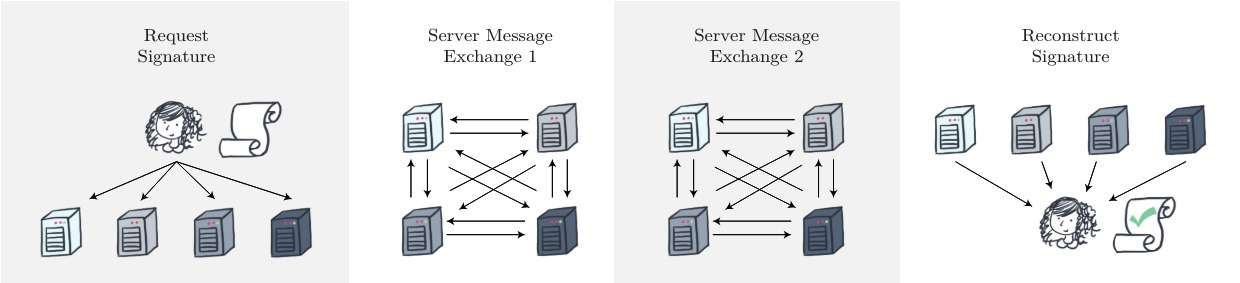
\includegraphics[width=0.95\textwidth]{threshold-signature.jpeg}
	\end{figure}
\end{frame}

\begin{frame}{Threshold Signatures}
	\vspace{-7mm}
	Issuer and its signing function replaced by an ideal functionality that computes same signing function when computed by the multiple servers.
	\vspace{4mm}
	\begin{block}{Security Properties}
		Threshold signing protocol (with threshold \textit{t}) with security against malicious adversaries \textit{under composition}\footnotemark:
		\begin{itemize}
			\item Same security properties as single honest issuer even if $t-1$ servers are compromised.
			\item No properties of credential need to be reproven if signing protocol is composible.
		\end{itemize}
		% Hence the paper now focuses on composably thresholdizing the BBS+ signature scheme.
	\end{block}
	\footnotetext{Universal Composability (UC) framework - R. Canetti, “Universally composable security: A new paradigm for cryptographic protocols,” in Proceedings of the 42nd Annual Symposium on Foundations of Computer Science (FOCS), 2001}
\end{frame}

% \begin{frame}{Preliminaries}
% 	\begin{block}{Bilinear Pairings}
% 		Let $G$ and $G_T$ be groups of prime order $q$. A map $e : G \times G \rightarrow G_T$ must satisfy the following properties:
% 		\begin{itemize}
% 			\item \textit{Bilinearity}: a map $e : G \times G \rightarrow G_T$ is bilinear if $e(a^x, b^y)t = e(a, b)^{xy}$;
% 			\item \textit{Non-degeneracy:} for all generators $g, h \in G, e(g, h)$ generates $G_T$ ;
% 			\item Efficiency: There exists an efficient algorithm $BMGen(1^k)$ that outputs $(q, G, GT , e, g)$ to generate the bilinear map and an efficient algorithm to compute $e(a, b)$ for any $a, b \in G$.
% 		\end{itemize}
% 	\end{block}
% \end{frame}

\section{BBS+ Signature Scheme}
\begin{frame}{BBS+ Signature Scheme}
	\begin{itemize}
		\item Anonymous signature scheme using bilinear pairings.
		\item Allows signing multiple messages ($\ell$) at once.
		\item Size of signature independent of number of messages signed.
		\item Efficient ZKPoK that reveals selective attributes.
		\item Based on the q-Strong Diffie-Hellman (qSDH) assumption.
	\end{itemize}
\end{frame}

\subsection{Key Generation}
\begin{frame}{Key Generation}
	\begin{block}{BBS+Gen($\mathcal{G}, \ell $)}
		\begin{enumerate}
			\item $\mathcal{G} = (\mathbb{G}_1, \mathbb{G}_2, g_1, g_2, q)$
			\item $H = \lbrace h_0, h_1, \ldots, h_{\ell} \rbrace$, where $h_i \uar \mathbb{G}_1$
			\item $x \uar \mathbb{Z}_q^*$, $X = x \cdot g_2$
			\item $sk = (H, x)$, $pk = (H, X)$
			\item Return $(sk, pk)$
		\end{enumerate}
	\end{block}
\end{frame}

\subsection{Signing}
\begin{frame}{Signing}
	\begin{block}{BBS+Sign($sk, m \in \mathbb{Z}_q^{\ell}$)}
		\begin{enumerate}
			\item $sk = (H, x)$
			\item Nonces: $r \uar \mathbb{Z}_q$, $s \uar \mathbb{Z}_q$
			\item Compute:
			\begin{align*}
				A = \frac{g_1 + s \cdot h_0 + \sum_{i = 1}^{\ell} m_i \cdot h_i}{\colorboxed{red}{x + r}}
			\end{align*}
			\item Return $\sigma = (A, r, s)$
		\end{enumerate}
	\end{block}
\end{frame}

\subsection{Verification}
\begin{frame}{Verification}
	\begin{block}{BBS+Ver($pk,\, \sigma, m \in \mathbb{Z}_q^{\ell}$)}
		\begin{enumerate}
			\item $pk = (H, X)$, $\sigma = (A, r, s)$
			\item Check:
			\begin{align*}
				e(A, X + r \cdot g_2) = e(g_1 + s \cdot h_0 + \sum_{i = 1}^{\ell} m_i \cdot h_i, g_2)
			\end{align*}
			\item Output 1 if and only if equality holds.
		\end{enumerate}
	\end{block}
\end{frame}


\section{Thresholdizing the BBS+ Protocol}
\subsection{High Level Overview}
\begin{frame}{Threshold BBS+ Protocol}
	\begin{block}{High Level Overview}
		\begin{itemize}
			\item Main difficulty is that the signing involves computing the inverse of secret value $(x + r)$.
			\item Tackled using Bar-Ilan and Beaver secure inversion technique.\footnotemark
			\item Three phases:
			\begin{itemize}
				\item \textbf{Key Gen:} Initial setup and distribution of secret shares of $x$.
				\item \textbf{Signing:} Client chooses $t$ servers and gets signature share $A_i = (R_i, u_i)$ from each, which it combines and verifies to get final signature.
				\item \textbf{Verification:} Same as original BBS+ verification.
			\end{itemize}
		\end{itemize}
	\end{block}
	\footnotetext{Bar-Ilan, O., Beaver, D.: Non-cryptographic fault-tolerant computing in constant number of rounds of interaction. In: Proceedings of the 20th Annual ACM Symposium on Theory of Computing, pp. 201-209. ACM (1988)}
\end{frame}

\subsection{Key Generation}
\begin{frame}{Key Generation}
	\begin{enumerate}
		\item Share of the secret key $x_i$ for party $\mathcal{P}_i$: % Shamir secret sharing of a random value.
		\begin{itemize}
			\item $\hat{x}_i(\cdot) \uar (t-1)$ degree polynomials. 
			\item Send $\hat{x}_i(j)$ to every party $\mathcal{P}_j,\ j \neq i$.
			\item $x_i = \sum_{j=1}^{n} \hat{x}_i(j)$.
		\end{itemize}
		\item Public key share $X_i = x_i \cdot g_2$.
		\begin{itemize}
			\item Commit-and-release and ZKPoK of discrete log as correctness checks. % Check all X_i subsets lie on same polynomial.
		\end{itemize}
		\item Public key $X = x \cdot g_2$: found by taking any size $t$ subsets of $X_i$s. 
		\item $H$: Commit-and-release of random $\mathbb{G}_1$ elements.
		\item Output $pk = (H, X)$
	\end{enumerate}
\end{frame}

\subsection{Signing}
\begin{frame}{Signing}
	Client $\mathcal{C}$ approaches $t$ servers to sign on message $m$.
	\begin{enumerate}
		\item Using standard secret sharing, the $t$ signing parties agree on random values $c, r, s$, with each party having share $c_i, r_i, s_i$.
		\item The signing parties perform secret sharing of $u = c \cdot (x + r)$
		% \begin{itemize}
		% 	\item 
		% \end{itemize}
		\item Each party $\mathcal{P}_i$ can now compute \vspace{-5mm}
		\begin{align*}
			R_i = c_i \cdot (g_1 + s \cdot h_0 + \sum_{i = 1}^{\ell} m_i \cdot h_i, g_2)
		\end{align*} \vspace{-5mm}
		\item Client can now compute the signature using the shares $(R_i, u_i)$ as:
		\begin{align*}
			A = \frac{\sum_i R_i}{\sum_i u_i} = \frac{c \cdot (g_1 + s \cdot h_0 + \sum_{i = 1}^{\ell} m_i \cdot h_i)}{c \cdot (x + r)}
		\end{align*}
	\end{enumerate}
\end{frame}

\section{Weak Partially-Blind Signing}
\begin{frame}{Weak Partially-Blind Signing}
	Client does not send $m$ to the signing parties. Instead:
	\begin{enumerate}
		\item $\mathcal{C}$: Masking nonce = $s_0 \uar \mathbb{Z}_q$
		\item $\mathcal{C}$: Computes and sends (along with ZKPoK of $s_0$) \vspace*{-4mm}
		\begin{align*}
			B' = s_0 \cdot h_0 + \sum_{i = 1}^{\ell} m_i \cdot h_i
		\end{align*}
		\item $\mathcal{P}_i$: Determines $s$ as usual, and computes \vspace*{-3mm}
		\begin{align*}
			B = g_1 + s \cdot h_0 + B'
		\end{align*}
		\item $\mathcal{C}$: Computes final signature as $\sigma = (A, r, s + s_0)$
	\end{enumerate}
\end{frame}

\section{Applications}
\begin{frame}{Applications}
	\begin{itemize}
		\item The weak patially-blind signing protocol can be used to \textbf{coalesce multiple credentials} into a single compact credential.
		\item The thresholdizing technique can be used for other similar signature schemes, such as Verifiable Random Function (VRF) scheme.
		\item The scheme can be extended to support \textbf{strong blind signatures} with some added computational complexity. 
	\end{itemize}
\end{frame}

\section{Implementation and Benchmarks}
\begin{frame}{Implementation and Benchmarks}
	\begin{itemize}
		\item The authors implemented the protocol in Rust. (6400 LOC!)
		\item They run the simulations for different server counts - $n$ and different network environments - local, LAN, WAN.
		\item They also compare their benchmarks against other previous anonymous threshold signatures.
	\end{itemize}
\end{frame}

\begin{frame}{Results}
	% 2 images side by side
	\begin{figure}%
		\centering
		\subfloat[\centering Signing time vs n]{{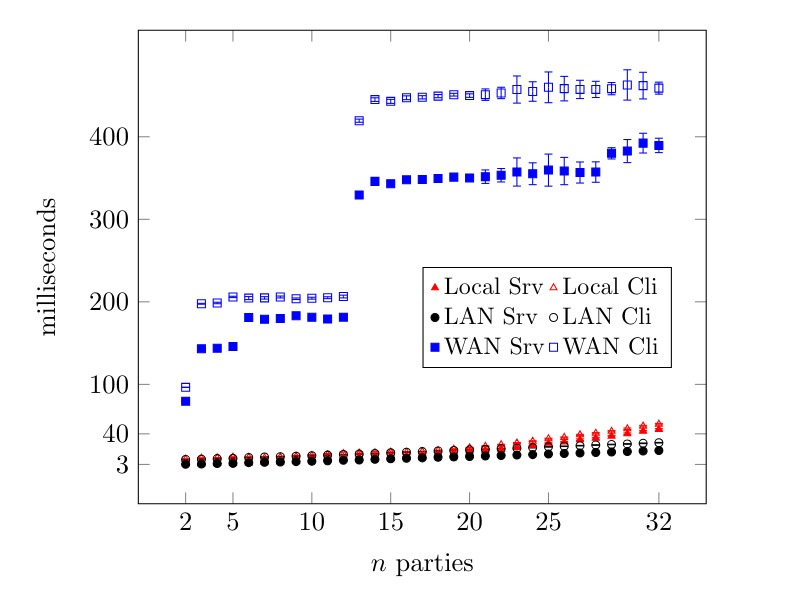
\includegraphics[width=5.5cm]{bbs.jpeg} }}%
		\qquad
		\subfloat[\centering BBS+ vs RP-Coconut]{{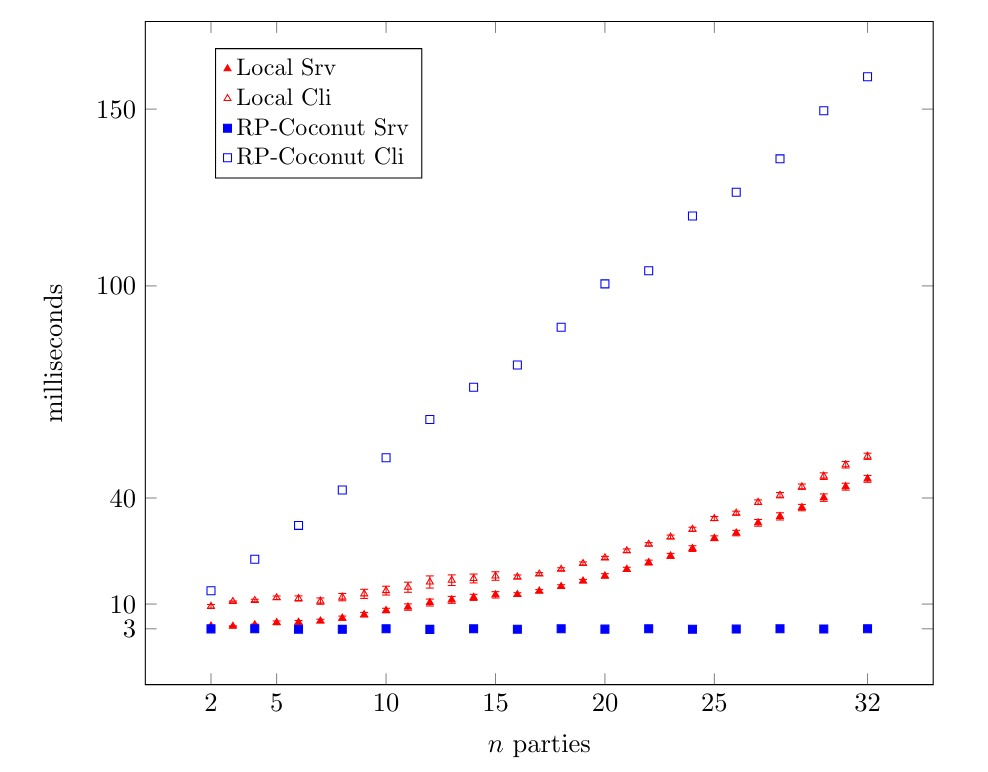
\includegraphics[width=5.1cm]{bbs-vs.jpeg} }}%
		\label{fig:example}%
	\end{figure}
\end{frame}

% \subsection{Tickets and Queues}
% \begin{frame}{Tickets and Queues}
% 	\begin{itemize}[<alert@+>]
% 		\item The user picks a ticket uniformally at random from the set of primes of atmost $l_t$ bits, where $l_t$ is 166. 
% 		\item As there are atleast $2^{160}$ tickets, the probability of two randomly chosen tickets colliding is atmost $2^{-80}$.
% 		\item We represent the queue maintained by the user as
% 		\vspace*{-3mm} $$Q = \{t_0, t_1, \dots, t_{k-1}\}$$
% 	\end{itemize}
% \end{frame}

% \subsection{Accumulator Scheme for Tickets}
% \begin{frame}{Accumulator Scheme for Tickets}
% 	\begin{itemize}[<alert@+>]
% 		\item We require that the users should be able to successfully prove that they have not been blacklisted by the IA, without revealing their tickets.
% 		\item Hence for this, we make use of Universal Dynamic Accumulators (UDAs), introduced by Li et al, which allows for an efficient ZKPoK of non-membership in time independant of number of accumulated values.
% 	\end{itemize}
% \end{frame}
% \begin{frame}{Accumulator Scheme for Tickets}
% 	The accumulator has a value V when values $S_T = \{ t_0, t_1, \dots, t_T \} $ are accumulated in it. We can perform the following operations with the help of the accumalator: 
% 	\begin{itemize}[<alert@+>]
% 		\item  $Accumulate(V, t_k)$ which outputs the updated value of the accumulator $V'$ that now also contains $t_k$.
% 		\item Each ticket $t$ not in $S_T$ has a corresponding non-membership witness $w$, such that $IsNonMember(t, V, w) = 1$ holds.
% 		\item This $w$ can be computed using knowledge of the secret key of the accumulator using $ComputeWitness(t, V, sk_{acc})$.
% 		\item Given (t, w) for an accumalator value V, anyone can update the witness w to a new witness w' for the updated accumulator value V' using $UpdateWitness(w, t, V, V')$.
% 	\end{itemize}
% \end{frame}

% \subsection{Protocol for Queue Signing}
% \begin{frame}{Protocol for Queue Signing}
% 	\begin{itemize}[<alert@+>]
% 		\item The RSU needs to verify the integrity of the queue, since otherwise a user could circumvent revocation by fabricating a queue with an incorrect set of K tickets.
% 		\item For this, normal digital signatures are not sufficient, as they will immediately allow the RSU to link the user to past actions. 
% 		\item We require the verification to happen without revealing either the queue or the signature on it.  
% 		\item For this, we utilize the signature scheme given by Camenisch and Lysyanskaya for a block of messages, adapted for our scheme.
% 	\end{itemize}
% \end{frame}

% \begin{frame}{Protocol for Queue Signing}
% 	This signature scheme allows us to perform the following necessary operations and ZKPoKs: 
% 	\begin{itemize}[<alert@+>]
% 		\item \textbf{Proof of knowledge of a signed queue: } This protocol allows a user to prove to the RSU the possession of a valid signature without revealing the queue and signatures themselves. 
% 		\item \textbf{Proof of relation between two queues: }
% 		\begin{itemize}
% 			\item During authentication, the user updates his queue from $Q$ to $Q' = Q.Enq(t_k).Deq()$ for use during the next authentication.
% 			\item This proof allows the user to convince to the RSU that $Q'$ was indeed correctly updated from $Q$.
% 		\end{itemize}
% 	\end{itemize}
% \end{frame}

% \section{Modified Scheme Construction}
% \begin{frame}{Modified Scheme Construction}
% 	Using the above mentioned building blocks, we can construct a modified scheme as follows:
% 	\begin{block}{Setup}
% 		\begin{itemize}
% 			\item For the randomizable signatures using bilinear pairings, the IA chooses a Type-3 pairing with the parameters $(e, g_1, g_2, g, G_1, G_2, G)$, and $(sk, pk) = ((x, y), (X=g_2^x, Y=g_1^y))$, where $x, y \in \mathbb{Z}_q^*$
% 			\item Depending on the system requirements, the IA decides on an appropriate revokation window size $K$. For our scheme, small values of $K$, such as $K=10$, would also be sufficient.
% 			\item The IA also initializes the accumalator, blacklist, and the parameters of the signature scheme for the queue.
% 		\end{itemize}
% 	\end{block}
% \end{frame}

% \begin{frame}{Modified Scheme Construction}
% 	\begin{block}{Registration}
% 		\begin{itemize}
% 			\item The user has secrets $(\alpha, \beta) \in_R \mathbb{Z}_q^*$, and sends $req = (a = g_1^{\beta}, b = a^{\alpha})$ to the IA. The IA verifies the user and outputs the signature $\sigma = (a, b, c = a^x, d = (bc)^y)$ to the user.
% 			\item Also the user picks a random ticket $t$ and initializes his queue as $ Q = \{ \hat{t}, \hat{t}, \dots, \hat{t}, t \} $, where $\hat{t}$ is a dummy ticket provided by the IA.
% 			\item Then the user engages in the ZKPoKs to prove his queue is well formed, and to get the witness for the ticket and signature for the queue.
% 			\item Finally, the user stores his credentials as \vspace*{-2mm}
% 			$$ cred = (\sigma, t, Q, (w_i)_{i=0}^{K-1}, \sigma', BL, V) $$
% 		\end{itemize}
% 	\end{block}
% \end{frame}

% \begin{frame}{Modified Scheme Construction}
% 	\vspace*{-2mm}
% 	\begin{block}{Authentication}
% 		\begin{itemize}
% 			\item \textbf{Randomizable Signature check: } The user shares $\sigma^r = (a^r, b^r, c^r, d^r)$, which the RSU verifies by checking that $e(a^r, X) = e(c^r, g_2)$ and $e(d^r, g_2) = e(bc^r, Y)$.
% 			\item \textbf{Blacklist Check: } The user obtains the current blacklist from the RSU, and verifies that he hasn't been revoked.
% 			\item \textbf{Request for authentication: } 
% 			\begin{itemize}
% 				\item Using the updated value of the blacklist, the user updates the witness for each ticket in his queue, and generates a fresh ticket $t^*$.
% 				\item Then he engages with the RSU in the ZKPoKs to prove that his queue is well formed, and that none of his tickets have been revoked.
% 			\end{itemize}
% 			\item \textbf{Refreshment issuing: } After verifying the user, the RSU computes the witness and signature for the queue, and sends it to the user.
% 			\item \textbf{Credential Refreshment: } Finally the user updates his credentials for the next authentication using the signature and witness.
% 		\end{itemize}
% 	\end{block}
% \end{frame}

% \begin{frame}{Modified Scheme Construction}
% 	\begin{block}{Revocation}
% 		\begin{itemize}
% 			\item To blacklist a misbehaving user who provided $t_k$, the RSU/IA updates the blacklist as $BL' = BL \cup \{ t_k \}$, and updates the accumulator as $V' = Accumulate(V, t_k)$.
% 			\item The next time the misbehaving user tries to authenticate, he will be unable to prove that $t_k$ from his queue is not in the accumulator. Hence he won't be authenticated.
% 		\end{itemize}
% 	\end{block}
% 	\begin{block}{Key generation and Encryption Scheme}
% 		After the authentication in the above steps, the rest of the construction for key generation and sharing of encrypted CAMs can be done similarly to the original scheme.
% 	\end{block}
% \end{frame}

\begin{frame}
	\begin{center}
		\huge Thank you!
	\end{center}
\end{frame}

\end{document}